\documentclass[11pt]{article}
\usepackage{amsmath,amssymb,graphicx}
\usepackage[margin=1in]{geometry}
\title{An exact finite-range benchmark for TD-SCHA interpolation}
\author{}
\date{}
\begin{document}
\maketitle

\paragraph{Model.}
Use a one-dimensional chain of molecular internal displacements $x_n$,
with mass, lattice spacing and $\hbar$ equal to one. These are optical
relative coordinates; a decoupled centre-of-mass acoustic chain can be
added to obtain a translationally invariant molecular crystal.
Take the fixed auxiliary dispersion
\[
 D(q)=1+0.8\cos(2\pi q),\qquad \omega_q=\sqrt{D(q)}.
\]
The minimum frequency is $\sqrt{0.2}$, so the reference is positive definite.
Define $s_{a,n}=\sum_r h_{a,r}x_{n+r}$ with
\[
 h_3=(1,0.35),\quad h_{4a}=(1,0.37,-0.29,0.21),
 \quad h_{4b}=(1,-0.23).
\]
An explicit bounded polynomial potential is
\begin{align*}
 V={}&\frac12\sum_{nm}x_nD_{n-m}x_m
 +\frac{g}{6}\sum_n(s_{3,n}^3-3C_3s_{3,n})\\
 &+\sum_{a=4a,4b}\frac{\lambda_a}{24}
 \sum_n(s_{a,n}^4-6C_as_{a,n}^2+3C_a^2),\\
 &g=0.5,\qquad \lambda_{4a}=0.72,\qquad\lambda_{4b}=0.24.
\end{align*}
The largest cluster spans three lattice spacings and contains four
distinct cells. Positive quartic coefficients make the model bounded
below: in particular $h_{4b}(q)$ has no zeros, so its quartic sum controls
all displacement directions in any finite periodic cell.

\paragraph{Precisely what is held fixed.}
Choose $N_c=9$, temperature $T=0$, and compute the constants once:
\[
 C_a=\frac1{N_c}\sum_{q\in\mathcal Q_c}
 |h_a(q)|^2\frac{1}{2\omega_q},\qquad
 h_a(q)=\sum_r h_{a,r}e^{2\pi iqr}.
\]
The subtractions cancel the average anharmonic force and curvature in
that coarse Gaussian. Freeze these coefficients and $D(q)$ when increasing
the mesh. Do not minimize SSCHA again and do not retune the counterterms.
The fine Gaussian generally has different $C_a^{(f)}$; its additional
average curvature would contain
$\sum_a\lambda_a(C_a^{(f)}-C_a)|h_a(q)|^2/2$.
This is the finite-mesh change of the quartic loop contribution that is
deliberately excluded from the benchmark. A fixed auxiliary matrix already
contains its reference renormalization; fixing it does not remove all
previously incorporated loop physics.

\paragraph{Independent exact vertices.}
At zero centroid, averaging the third derivative of the quartic terms
gives zero, and the fourth derivative is constant. Thus both vertices
are independent of the change of Gaussian covariance:
\[
 \Phi^{(3)}(q_1,q_2,q_3)=g\prod_j h_3(q_j),\qquad
 \Phi^{(4)}(q_1,q_2,q_3,q_4)=\sum_a\lambda_a\prod_j h_a(q_j),
\]
with total momentum conserved. In the ordered pair convention of the
reference implementation, define
\[
 v_k=\frac{\Phi^{(3)}(-k,k-Q,Q)}{\sqrt N},\qquad
 W_{kk'}=\frac{\Phi^{(4)}(-k,k-Q,k',Q-k')}{N}.
\]
The diagonal pair propagator $\Lambda$ includes the identical-pair factor
of $1/2$. Compare
\[
 \Sigma_B=v^\dagger\Lambda v,\qquad
 \Sigma_R=v^\dagger(I-\Lambda W)^{-1}\Lambda v,\qquad
 G=[z^2-D(Q)-\Sigma]^{-1}.
\]
Switch off $W$ only in the response calculation to obtain the bubble
control; do not change the potential or auxiliary matrix. A purely even
quartic potential at zero centroid would instead give $v=0$ and no
bubble-mediated change of this one-phonon response. The cubic term is
therefore essential. Pure-quartic isolation should test the pair response.

\paragraph{Exactness argument.}
At fixed external $Q$, the dependence of each quartic pair leg on its
internal momentum is a trigonometric polynomial supported on
$r=-3,\ldots,3$. On an odd coarse mesh, $N_c>2\times3$ is sufficient
for unique centered Fourier reconstruction. Merely requiring the cell
length to exceed three is insufficient. With the cardinal interpolation
matrix $P$,
\[
 v_f=\sqrt{N_c/N_f}\,Pv_c,\qquad
 W_f=(N_c/N_f)PW_cP^\dagger.
\]
Consequently the reconstructed and directly evaluated fine vertices
are identical. Using the same fine $D$, pair quadrature, $z$ and temperature
makes both bubble and fully resummed responses identical wherever their
resolvents exist. This proves exactness within the chosen TD-SCHA/RPA
response, not exactness relative to the full anharmonic quantum problem.
No finite-support assertion is made about $G$ or $\Sigma$ themselves.
The current production implementation refines internal loop momenta;
external $Q$ must remain on the coarse mesh.

\paragraph{Measured example and paper figures.}
The companion \texttt{paper\_model.py} evaluates $9\to72$ cells at $Q=0$,
$T=0$, $z=\omega+0.015i$, over $0.6\leq\omega\leq1.65$.
Direct and interpolated bubble/RPA responses agree to below $10^{-14}$
in relative Euclidean norm. Quartic resummation changes the spectral
curve $-\operatorname{Im}G/\pi$ by $37.7\%$ in that norm and the
self-energy by $42.7\%$. The sampled dominant maximum moves from
$1.2975$ to $1.3100$. Minimum static curvatures sampled on 72 momenta
are $0.1826$ (bubble) and $0.1846$ (RPA). These diagnose local stability
on the sampled grid, not global thermodynamic stability.
\begin{center}
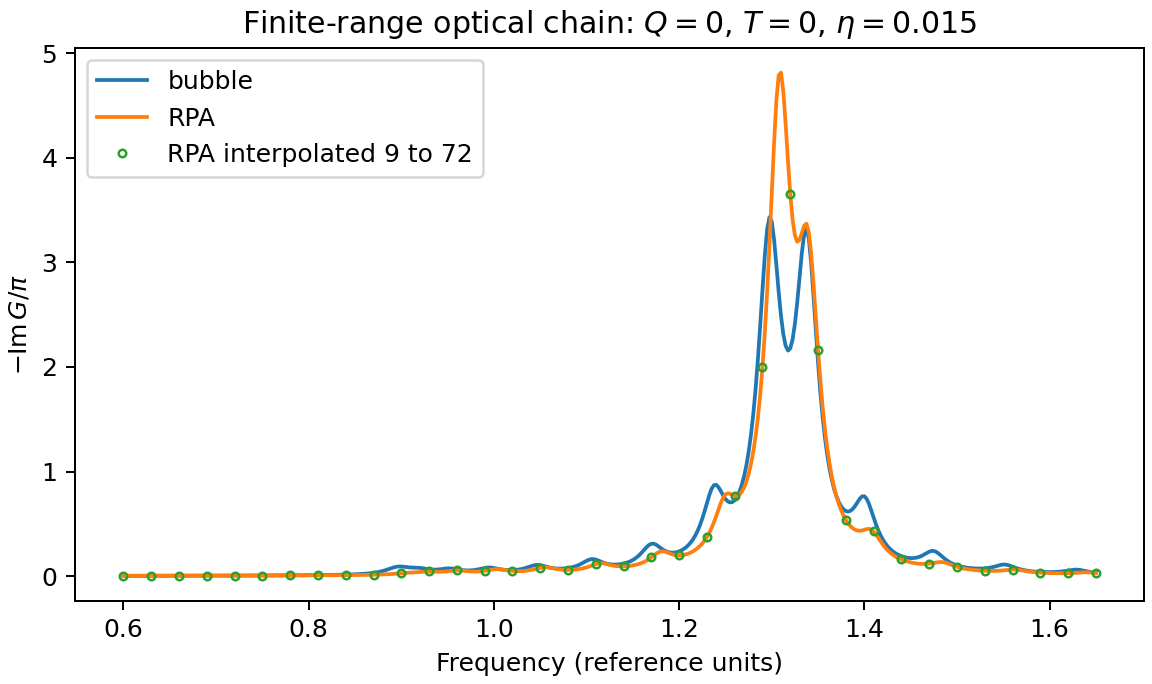
\includegraphics[width=.9\linewidth]{paper_model_spectrum.png}
\end{center}
For a paper, show (i) direct versus interpolated bubble and RPA spectra,
(ii) interpolation errors against coarse size with an underresolved
negative control, and (iii) a separate fine-mesh and broadening convergence
study. The displayed finite-mesh peak structure must not be interpreted
as a converged lifetime. The existing production Gaussian-cubature tests
exercise actual force estimators without stochastic noise; the companion
script is an independent analytic calculation.

\paragraph{Formal reference.}
R. Bianco et al., Phys. Rev. B \textbf{96}, 014111 (2017),
doi:10.1103/PhysRevB.96.014111, provides the SSCHA free-energy-curvature
and higher-order resummation framework.
\end{document}
